% Created 2022-04-06 Wed 15:55
% Intended LaTeX compiler: pdflatex
\documentclass[a4paper, 11pt, twocolumn]{article}
\input{/home/casper/orgfiles/tex_templates/fun_article_template}
\usepackage[utf8]{inputenc}
\usepackage[T1]{fontenc}
\usepackage{graphicx}
\usepackage{longtable}
\usepackage{wrapfig}
\usepackage{rotating}
\usepackage[normalem]{ulem}
\usepackage{amsmath}
\usepackage{amssymb}
\usepackage{capt-of}
\usepackage{hyperref}
\usepackage{amsmath}
\usepackage{cleveref}
\newcommand{\m}[1]{\textbf{#1}}
\newcommand{\infdecay}{I(s_i : S^t)}
\usepackage{biblatex}
\addbibresource{/home/casper/library.bib}


\usepackage[english]{babel}
\author{Casper van Elteren}
\date{\today}
\title{An information theory perspective of tipping points in dynamical networks}
\begin{document}

\maketitle
\lettrineabstract{Abrupt, system-wide transitions can be endogenously generated by seemingly stable networks of interacting dynamical units, such as mode switching in neuronal networks or public opinion changes in social systems. However, it remains poorly understood how such `noise-induced transitions' are generated by the interplay of network structure and dynamics on the network. Here we use information theory to discover how such `'tipping points'' can emerge in dynamic networks governed by the Boltzmann-Gibbs distribution. We identify two key roles for nodes in for tipping behavior to occur. In the initial phase, nodes with low degree pass on short-lived fluctuations to neighboring nodes, causing a domino-effect making neighboring nodes more dynamic. Conversely, towards the tipping point we identify other nodes whose state information becomes part of the long-term memory of the system. In addition, we show that identifying the different roles enables performing different types of targeted interventions that make tipping points more (less) likely to begin or to lead to systemic change. In general this progression depends on the combination of network structure and dynamics, which can be discovered using our methodology. This opens up possibilities for understanding and controlling endogenously generated metastable behavior.}



\section{Introduction}
\label{sec:orgd6a1d62}
Multistability is an important characteristic in many real-world complex systems. It entails the phenomenon whereby a system under the influence of noise explore its state space on different timescales. For example, the neural network's of the brain can produce various oscillations that are different from their natural ground state \cite{Fries2015}. Similarly, the life cycle of a cell is tightly regulated between two bistable states of mitosis and interphase \cite{Kandel2000}. Other examples exist on larger scales such emergence of multistability in opinion dynamics, or the multistability of ecosystems or climate systems.  Multistability allows for a system to absorb and adapt to nose-induced fluctuations, yielding its universal character in many complex systems.

The mechanisms  underlying these  transitions are  often not well understood. It is of vital importance to understand the underlying  processes  that  cause  metastable  behavior  to quantify the impact of noise on complex systems.

Here, we  consider dynamical systems consisting of a static network where the states of the nodes are governed by a Boltzmann-Gibbs distribution. This type of model has been used to describe a wide range of behaviors such as  neural dynamics \cite{Hopfield1982b}, opinion dynamics,  ferromagnetic  spins \cite{Glauber1963}, and  organized criminal  gang  interactions  \cite{DOrsogna2015a}.

In this class of models, each node chooses its state in equilibrium with the potential induced by its neighboring states. In physical applications this potential is the classic energy potential, but in other applications it can be interpreted, for instance as frustrmation level, homophily, or more broadly speaking, a fitness score of the node state given its neighbors. The second ingredient in this model is a global `temperature' which is essentially a noise level: at zero noise a node always picks the absolute minimum energy state, whereas the higher this noise level, the more likely it is that high energy states are chosen.

For low noise levels, it is common for systems governed by the Boltzmann-Gibbs distribution to exibhit metastable behavior because of the existence of multiple (local) minima in the system's potential. In finite systems and non-zero temperature, there is a finite probability that the system moves (eventually) from one local minimum to another. Without loss of generality, in this paper we illustrate our method using the well-known kinetic Ising spin model without external forces. Here, nodes have only two possible states: +0 and +1. At system level, there are two global minima: all nodes in state +0 or all nodes in state +1. Between these two system states lies a `potential barrier': many possible paths of system states which connect the two systemic minima, but all of which have a growing potential, making these paths less likely than paths of similar length that remain close to one of the minima. The peak of this potential along each crossing path lies informally speaking at a `checkerboard pattern': each node being maximally different from (the majority of) its neighbors. We refer to this peak as the `tipping point'. See \cref{fig:introduction}.


The crucial point here is that the network structure can make systemic transitions much more likely than without it. Without network effects, each node has an independent probability of choosing the (unlikely) high potential state. The probability that all nodes in the system happen to do this simultaneously (thereby transitioning the system state to another potential minimum) decreases to zero rapidly (as $\mathcal{O}(e^{-N^2})$ for dense networks). This means that transitions become unlikely for all but the smallest systems. With network effects, however, transitions can potentially occur along a path of nodes that form a domino effect. That is, the first node choosing randomly a high potential state makes the same state transition more likely for all of its neighbors. For some of these neighbors this new situation may suffice to make the same transition with (almost) equal likelihood as the first node, and so on, until the tipping point has been reached. The likelihood of such a transition is much higher than without network effects (up to $\mathcal{O}(e^{-N})$). This is still an exponentially decaying function of system size, highlighting the fact that such noise-induced transitions still only occur in finite-size systems, but exceedingly more likely.


Here we present a  method   to    uncover the network percolation process that facilitates  endogenous,   noise-induced
transitions. The computational method only requires access to cross-sections of time-series of observations of the  system, meaning
that it is broadly applicable.

The method consists of analyzing two key features using information flows of a system: the time of the short-term information decay, and the long-term information level. Here, the contribution of each node to the system dynamics over time are considered. The results highlight that short-lived correlations measured by Shannon mutual information shared between and node and the entire system ($I(s_i : S^t$) are essential to absorb and transfer noise through the system. After the majority of the system crosses the tipping point, a new local equilibrium is established. These long-term correlations are essential for the system to maintain its metastable state.
The approach differs from traditional approaches that focus on how the system as a whole approaches a tipping point. Here, the mechanism underlying \emph{how} local connectivity of nodes contribute to the system dynamics can be understood and analyzed.

\begin{figure*}
\centering
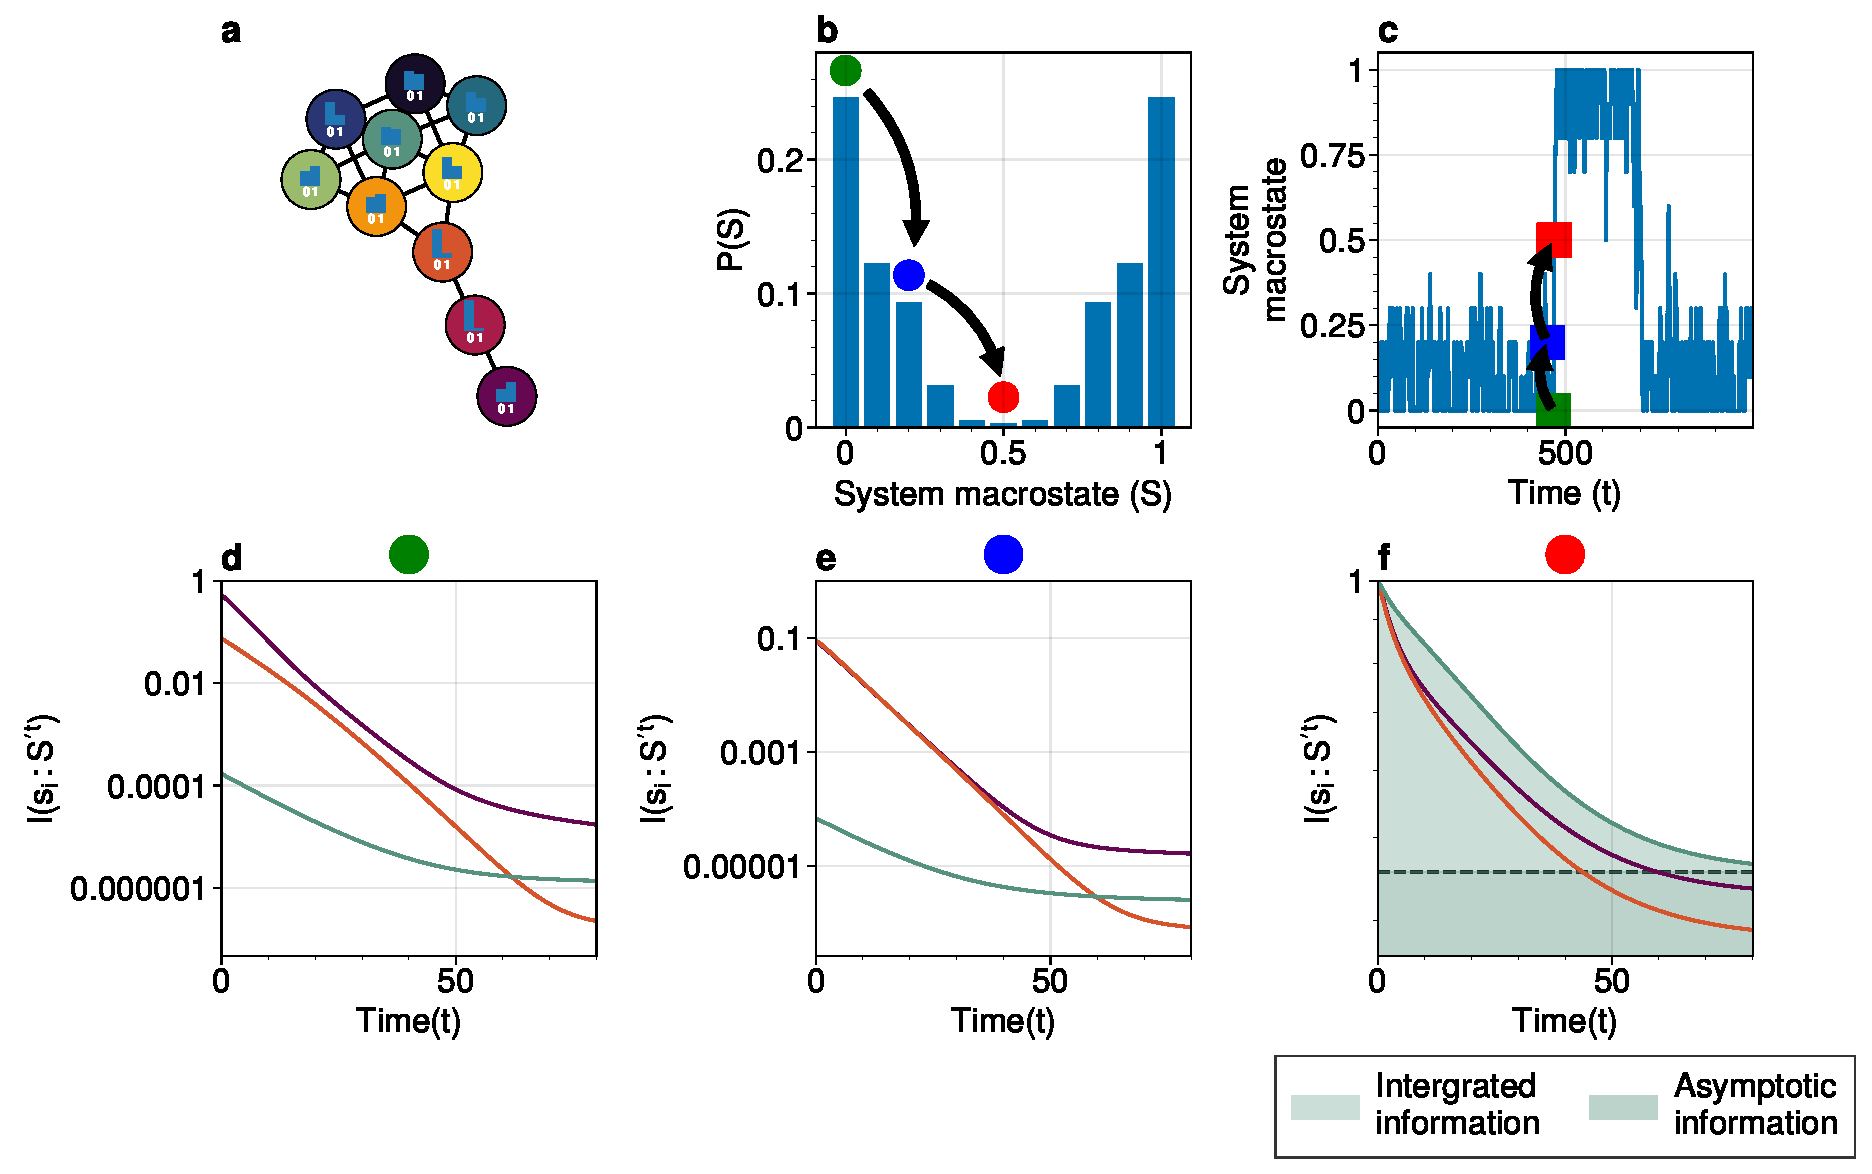
\includegraphics[width=0.9\textwidth]{./figures/figure1.pdf}
\caption{\label{fig:introduction}(a) A system consists of elements (circles) with a coupled interaction structure (edges). Each node has some intrinsic dynamics, indicated by the energy lines (gray); a low configurational energy corresponds with a ``stable'' state. Out of equilibrium the temporal dynamics of such a transition are depicted in (c). By studying the information flows as a function of tipping distance (d-f), The integrated mutual information represents the area under the curve for the information decay of a node with the system over time ($I(s_i : S^t)$): it is a measure of how much the current node state, predicts the future system state. Asymptotic information forms an approximation of long timescale dynamics. In contrast, the integrated mutual information captures the short timescale dynamics out-of-equilibrium. Shown are a selection of the information decay curves for 3 nodes from (a). Through information features, the mechanism underlying metastable transitions can be understood (d): far away from the tipping point, information processing occurs in low degree nodes, as the system approaches the tipping point (e, f), the higher degree nodes are recruited. The information cascade unravels the mechanisms whereby short-lived correlations are essential for priming the system for the metastable transition. For more information on numerical approaches see \ref{sec:org8193119}.}
\end{figure*}

\section{Results}
\label{sec:org6f0b033}

% leg de opzet van de studie uit
\Cref{fig:introduction}{a-c} shows a graphical representation of how a network of binary distribution governed by \cref{eq:glauber,eq:energy} can lead to bistability of the system macrostate. Some configurations of the system are more stable than other configurations (\cref{fig:introduction}{b}). Three markers are highlighted to show the transition between the system close to the ground state towards the tipping point. The circles indicate the set of states, whereas the squares correspond to a particular system state drawn from the bins corresponding to the circle of the same color.

In \cref{fig:introduction}{c} typical system trajectory is shown using Glauber dynamics. Note how most transient noise induced perturbations relax the system system back to the closest ground state. For some perturbations, however, the system moves rapidly from the stable regime (green square) towards the tipping point (red square).

The contribution of a node to the occurence of a tipping point is not equal. Consider for example a node with low degree, e.g. degree 1, and a node with high degree, e.g. degree 10 (\cref{fig:maj_flip}). A node with lower degree is more likely to flip given the state of its neighbors than a node with higher degree. Consequently, it is more likely that nodes with lower degree destabilize the system, pushing the system closer to the tipping point than a high degree node even though the contribution to the instantaneous macrostate is equal.

% Naar discussion
% By considering the system macrostate under the influence of two major forces, the mechanism underlying the tipping behavior is starting to show a remarkable structure. We distinguish destabilizer nodes as those nodes that are more likely to flip from the minority to the majority state. These nodes absorb and propagate noise into the system. Opposed are stabilizer nodes that prevent noise from being propagated through the system. These nodes are less likely to change their state under the influence of small perturbations.

From an information perspective, the contribution of the dynamics of a node can be quantified using time-delayed Shannon information. Depending on the connectivity of a node in the system, the contribution to the system macrostate will differ \cite{vanElteren2022,Quax2013}. How much the future system state is affected by the node's current state is computed by shared information with the node's current state $s_i$ and the future system state $S^t$ as the adjusted mutual integrated information

\begin{equation}
\label{eq:adj_imi}
\bar \mu_(s_i) = \sum_{t = 0}^\infty (I(s_i : S^t) - \omega_{s_i}) \Delta t.
\end{equation}

Intuitively $\mu(s_i)$ represents the transient dynamics of how much the influence of a node is "remembered" by the system over time. It reflects how the effects of local dynamics between nodes percolates through the system over time. As the system chooses it next metastable state, the system macrostate is dominated by transient dynamics. The next tipping point will be reached on a much longer time-scale. Consequently, $\omega$ quantifies the system returning to a stable system regime. For nodes with fast dynamics, $\mu(s_i)$ is generally high and $\omega_{s_i}$ would be generally low. Importantly, nodes that maximize $\mu(s_i)$ are driver nodes in systems in systems goverened by the Gibbs distribution\ref{vanElteren2022}.


In \cref{fig:introduction}{d-f} the information flows are computed that quantifies the contribution of a node on the future system state. The information flows are computed by considering the system in different states of stability (see \ref{sec:org8193119}). That is, the subset of states are selected such that states $S_{\gamma} = \{S' \subseteq S | M(S') = \gamma\}$ where $\gamma \in [0,1]$ is the fraction of nodes having state +1. By evolving all possible trajectories, the exact information flows are computed for $t=500$ steps. Asymptotic and integrated mutual information are estimated using regression (\ref{sec:org8193119}).


\begin{figure*}
\centering
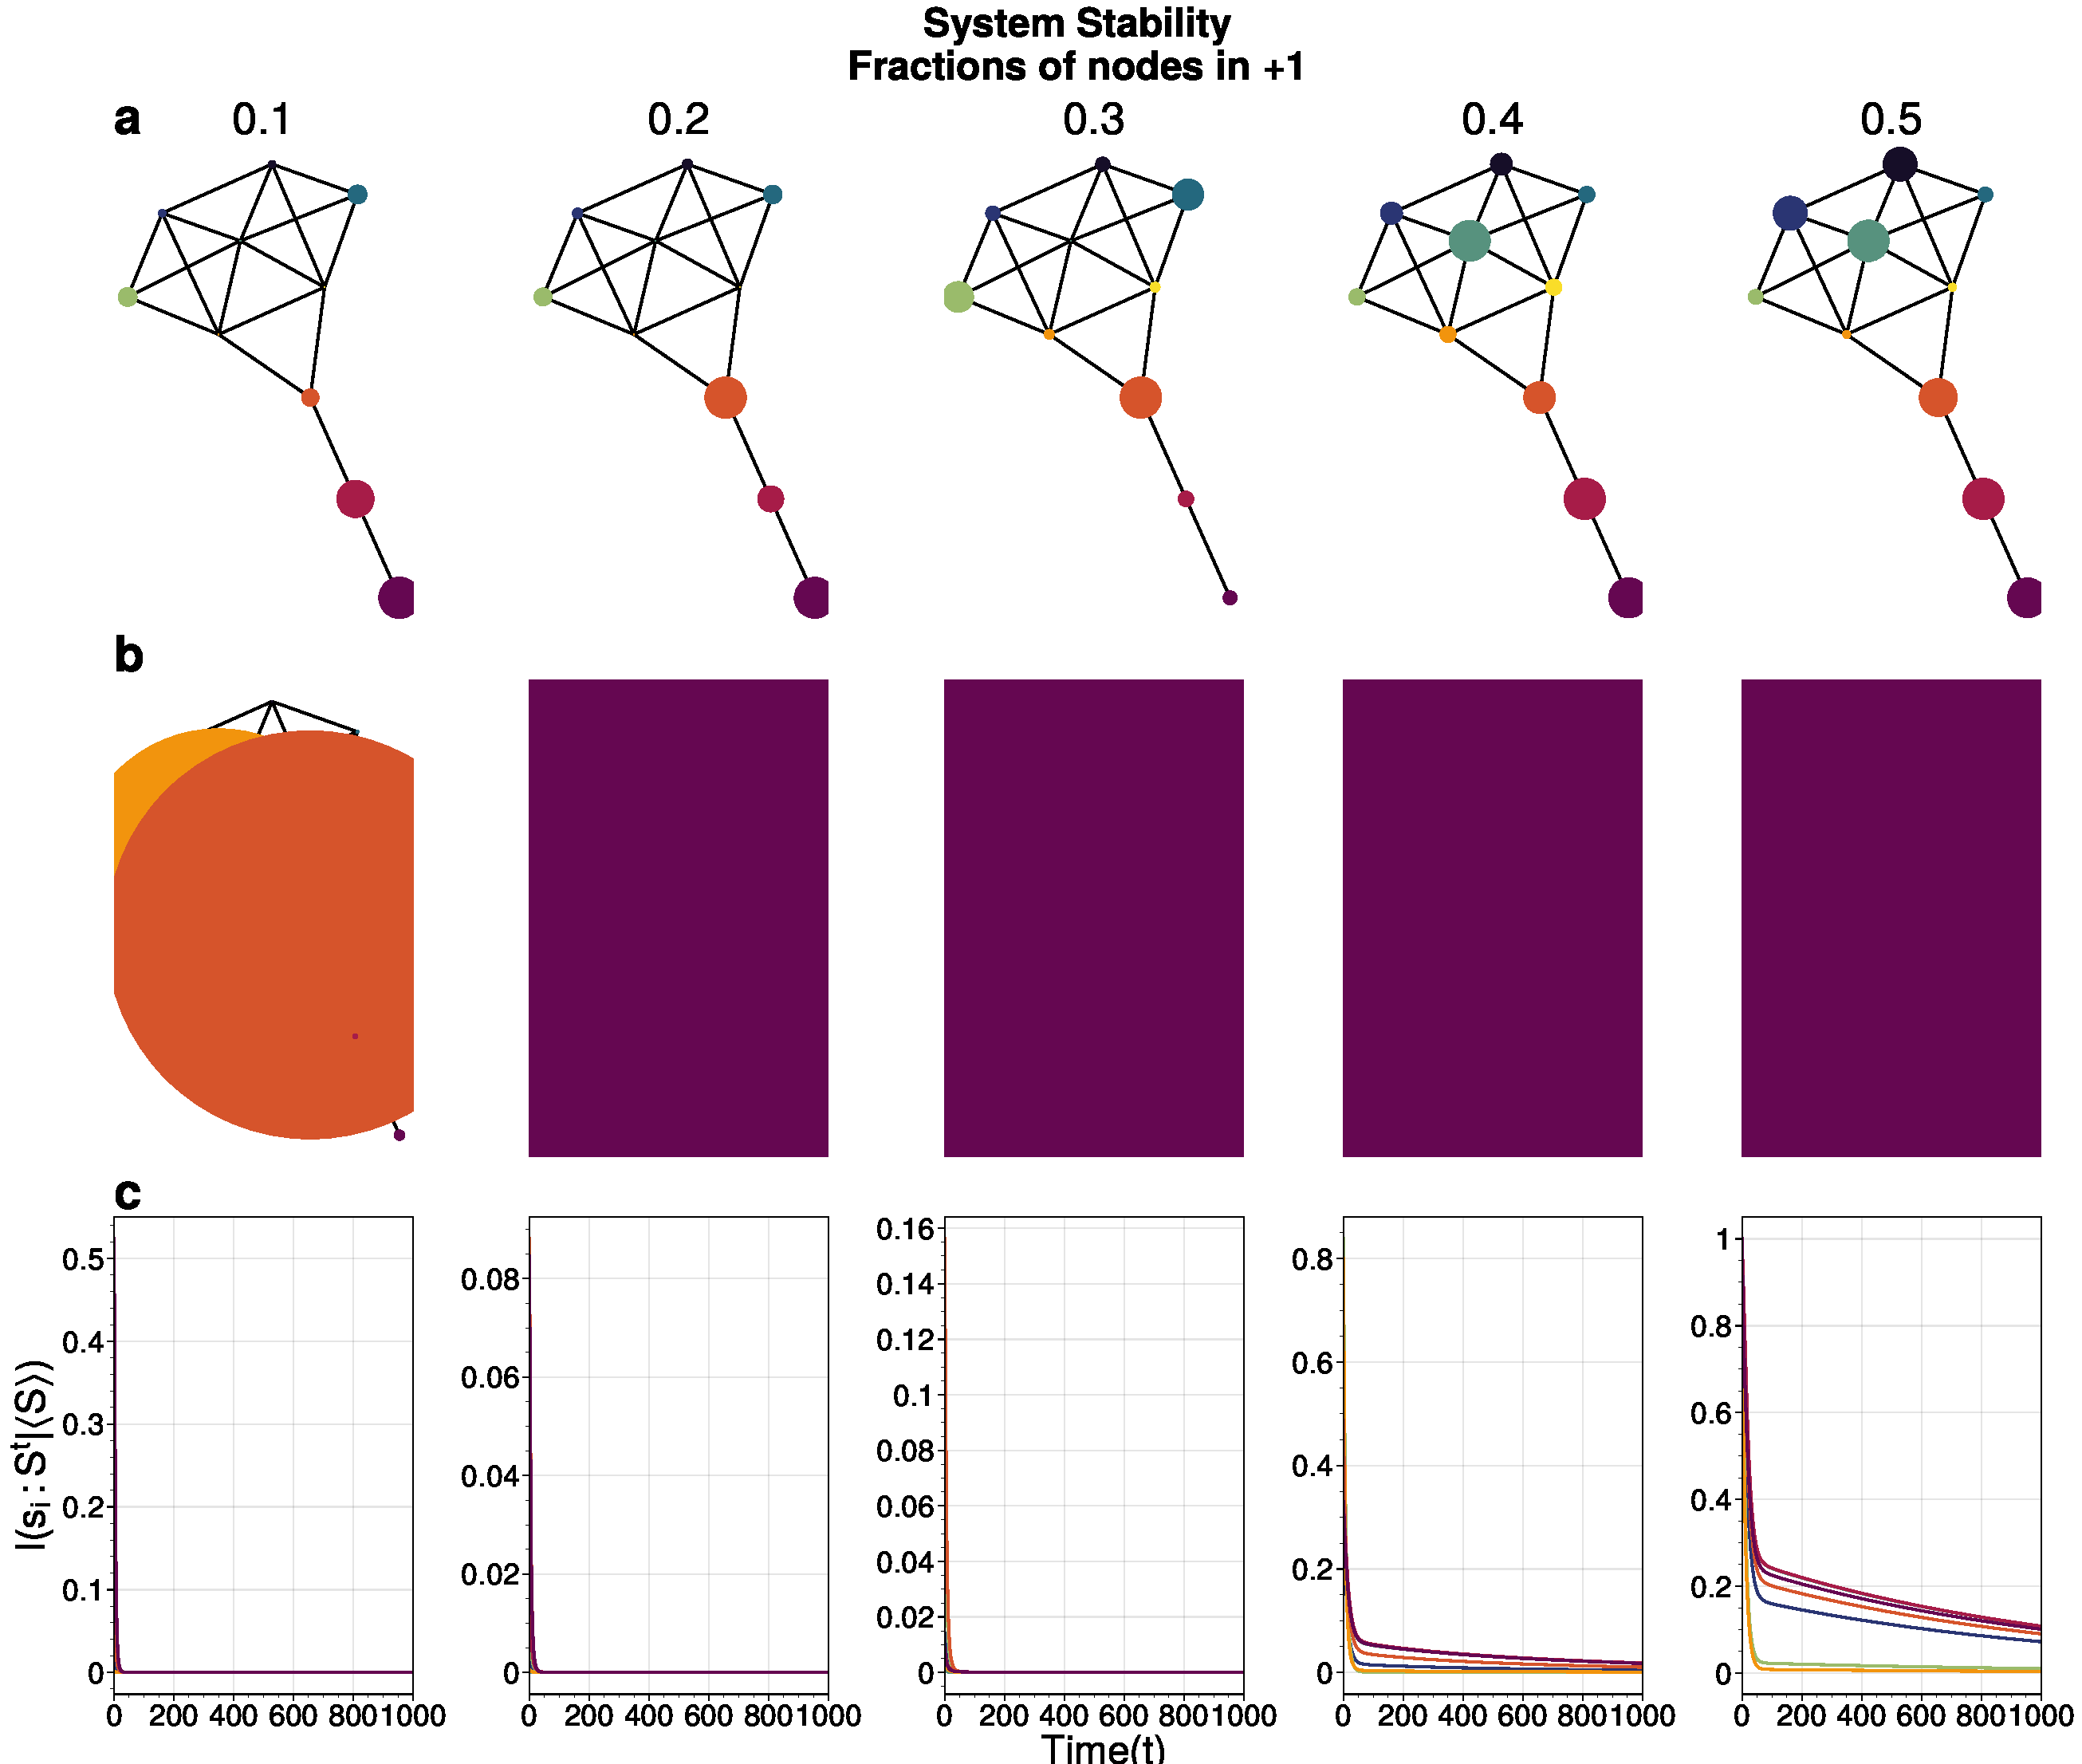
\includegraphics[width=.9\linewidth]{./figures/figure2.pdf}
\caption{\label{fig:kite_res}(a) As the system approaches the tipping point (left to right) the information processing moves from lower degree  nodes to higher degree nodes. Each node is governed by kinetic Ising dynamics updated by Glauber dynamics. The node size is proportional to the adjusted integrated mutual information in (a) and the asymptotic information in (b). (c) Far from the tipping point, the information processes are dominated by low degree nodes. As the system approaches the tipping point the asymptotic information maximizes and the fast-time scale dynamics becomes similar.}
\end{figure*}

Two things are observed. First, the tipping point is reached by a domino effect where low degree nodes flip first, and then causing neighboring nodes to flip. Far away from the tipping point (\cref{fig:kite_res}{a}), nodes with lower degree are causally more important (higher $\mu(s_i)$) than higher degree nodes. This can be understood by considering the likelihood of the node flipping as a function of degree and system macrostate (\cref{fig:maj_flip}). Lower degree nodes by definition have fewer constraints from nearest neighbor interactions, which makes flipping from the majority to minority states more likely than higher degree nodes. Consequently, lower degree nodes drive the system towards the tipping point by injecting noise into the system. As the system is further destabilized, the flip probability for higher degree nodes from majority becomes more likely and the driver node changes to higher degree nodes closer to the tipping point. In \cref{fig:max_trajectory} a trajectory is shown that maximizes $\log P(S^t|S^{t-1}, S^0 = \{0\}, M(S^5) = 0.5)$. The system starts in the stable regime with all nodes having state +0. The tipping point is reached by the lowest degree node flipping first, which promotes the probability of its neighbor flipping.

Second, an increase in asymptotic behavior indicates the system transitioned between metastable points. The asymptotic information remains low far away from the tipping point, and monotonically increases as the system approaches the tipping point (\cref{fig:introduction}{e, f} and \cref{fig:kite_res}{b}). The increase in a node's asymptotic information reflect how the system is more likely to transition between metastable points. That is, the system either relaxes to the closest ground state or transitions across the tipping point into the next metastable state. After such a transition, the dynamics of the nodes slow down. That is, all but the nodes with the lowest degrees are locally frozen as the system dynamics restabilizes after a noise-induced perturbation.

\begin{figure*}
\centering
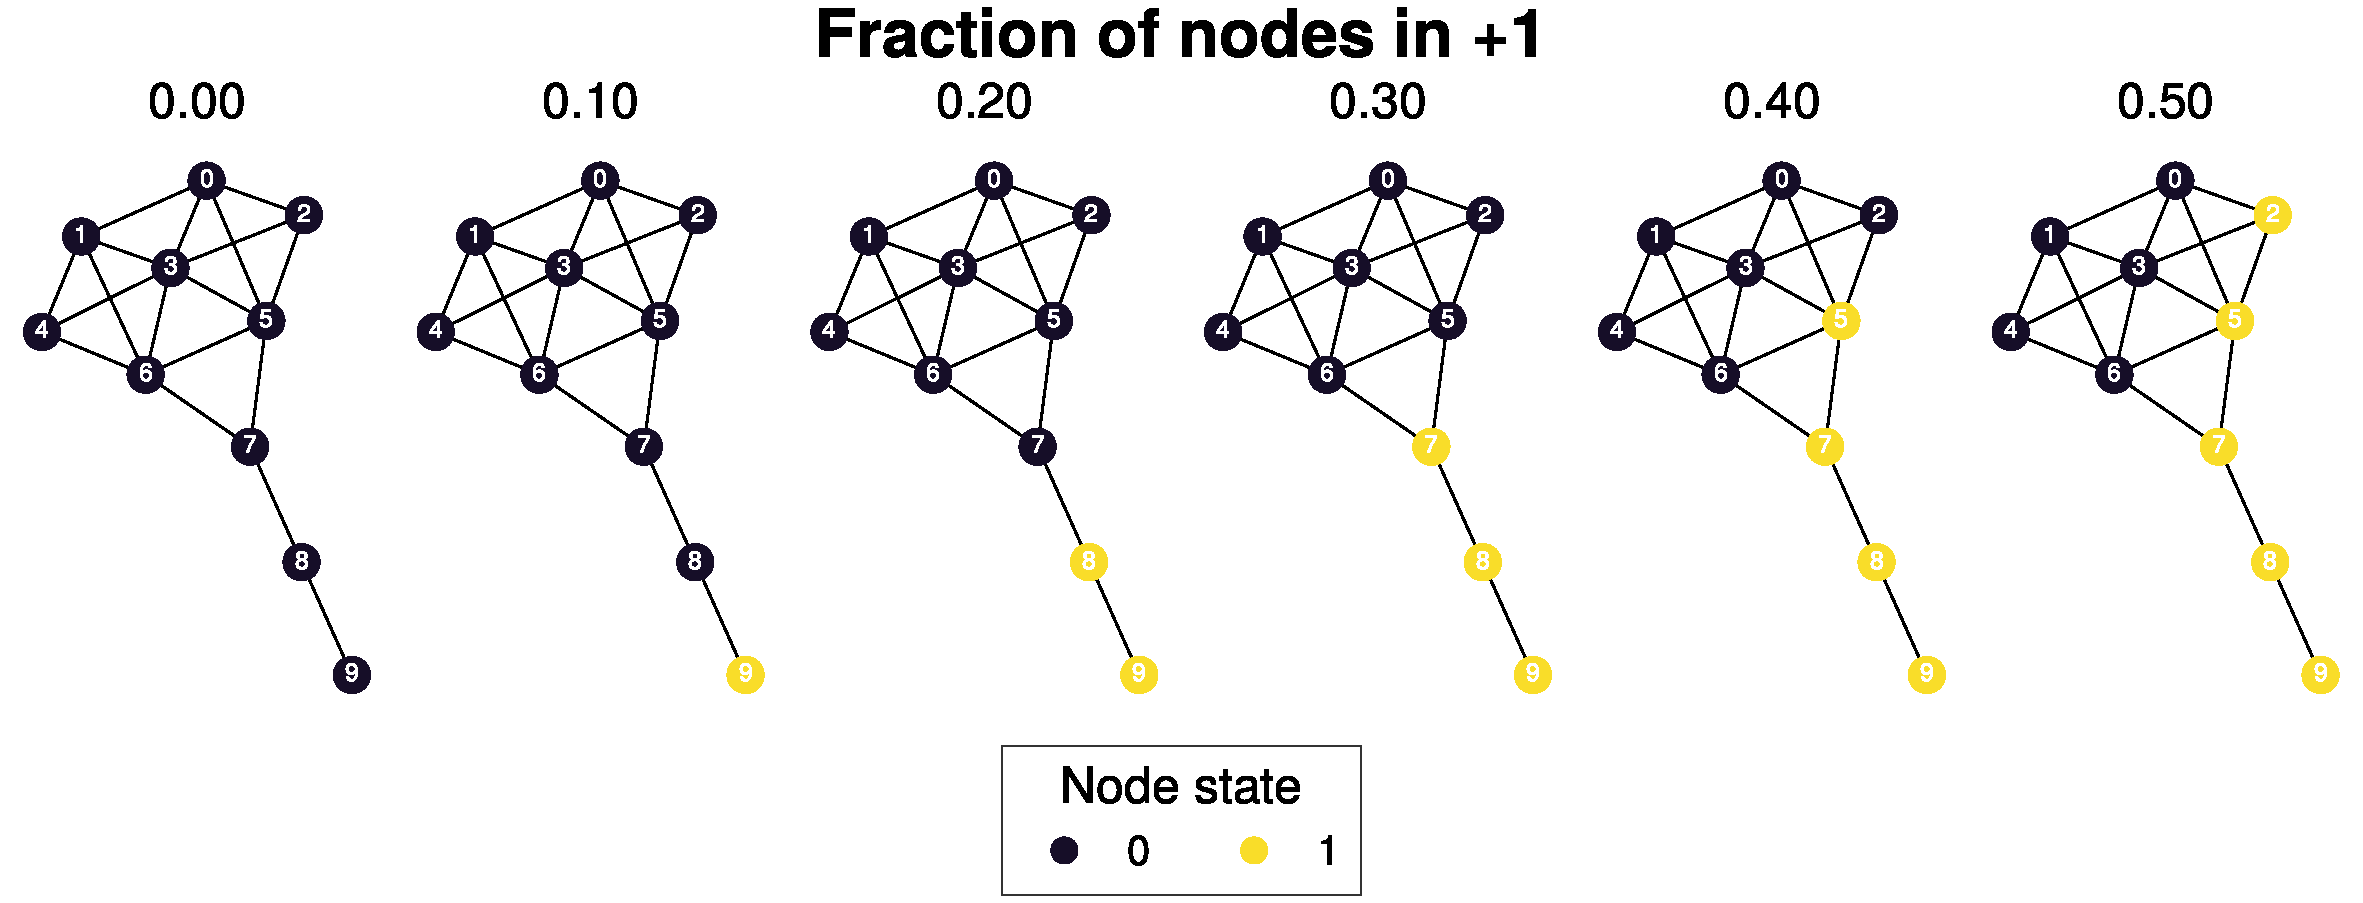
\includegraphics[width=.9\linewidth]{./figures/kite_maximized_trajectory_30230.pdf}
\caption{\label{fig:max_trajectory}The tipping point is initiated from the bottom up. Each node is colored according to state 0 (black) and state 1 (yellow) Shown is a trajectory towards the the tipping point that maximizes $\sum_{{t=1}}^{{5}} \log p(S^{{t-1}} | S^t, S^0 =\{0\}, M(S^5) = 0.5)$. As the system approaches the tipping point, low degree nodes flip first, and recruit ``higher'' degree nodes to further destabilize the system and push it towards a tipping point. There are in total 30240 trajectories that reach the tipping point in 5 steps, and there are 10 trajectories that have the same maximized values as the trajectory shown in this figure.}
\end{figure*}

\begin{figure*}
\centering
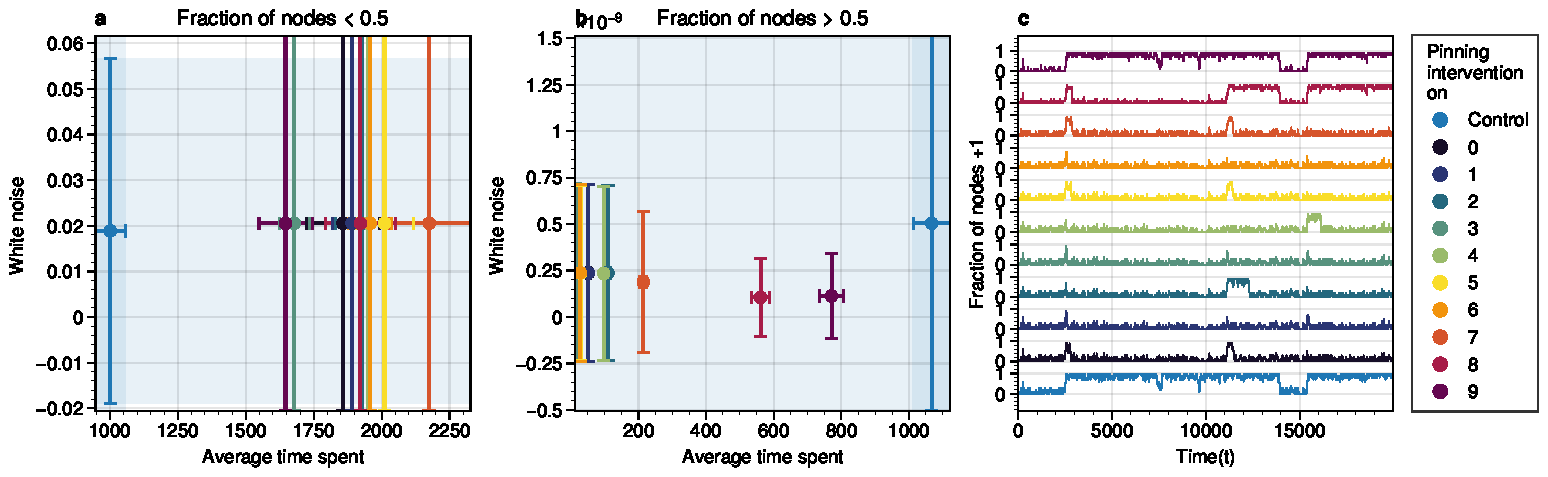
\includegraphics[width=.9\linewidth]{./figures/figure4.pdf}
\caption{\label{fig:kite_noise}White noise of the system macrostate outside the tipping point. Numerical simulations were performed using 6 different seeds. (a, b) White noise was estimated for the instantaneous system macrostate for the two stable point (a, b) (see \ref{sec:orgc093508}). The intervention pinned the node at state +0. This causes the system to prefer the macrostate where the fractions of nodes are < 0.5 regardless of the node intervened on. Importantly, the figure shows that intervention on the lower degree nodes (e.g. 9 or 8) removes high frequency noise (c). Compared to the control condition (blue bands) the interventions on higher degree nodes (e.g. 4) produces more white noise for the system macrostate but less frequent tipping points.  The high frequency noise is essential to initiate the metastable transition whereas higher degree nodes are essential to retain the stability when the tipping occured. Interventions on higher degree nodes prevents the tipping point from occurring as the higher degree nodes have to flip as the system crosses the tipping point. Interventions on higher degree nodes therefore produce higher levels of white noise for (a) but less for (b) as the system macrostate does not make the metastable state that often. (c) Shown are a system trajectory for the krackhardt kite graph with seed 1234. An intervention pins the node state at state +0. The figure shows that intervention on lower degree nodes remove high frequency noise (e.g. see node 9 or 8) when the system macrostate is below 0.5, but increased when the system is above 0.5. For lower degree nodes the system is more stable when the macrostate is below 0.5. In contrast, interventions on higher degree nodes (e.g. node 3), transitions less between metastable states but has increased noise when the system is <0.5.}
\end{figure*}

The cascade of flips is further studied using causal interventions (\cref{fig:kite_noise}). By pinning each node state to +0 in separate simulations, the effect on the occurrence of tipping points is studied. The interventions highlight two distinct roles for the metastable transitions. Intervention on low degree nodes removes the white noise in the system macrostate +0 but increases the white noise when the system reaches the macrostate +1. The effect is most prominent for node 9 which has degree 1 (\cref{fig:kite_noise}{c}); interventions on node 9 yields the lowest time spent in the +0 metastable state (\cref{fig:kite_noise}{a}), and the highest time spent in the +1 macrostate relative to interventions on other nodes(\cref{fig:kite_noise}{b}). Notable, the number of tipping transitions is the least affected by lower degree nodes. In contrast, high degree nodes seem to be essential for the tipping behavior to last. That is, lower degree nodes are necessary to destabilize the system, but the higher degree nodes have to flip in order for the new metastable state to endure. This can be seen by the time spent in the +1 macrostate: interventions on a hub nodes has increased white noise compared to control conditions in the +0 macrostate (\cref{fig:kite_noise}{a}). This indicates that noise is propagated and nodes are flipped towards the tipping point, but are less likely  to cross the tipping point. This is further strengthened by the reduced time spent in the +1 macrostate as a function of degree \cref{fig:kite_noise}{b}.

Lastly, the relative difference between integrated mutual information is the lowest at the tipping point. At the tipping point, the relative contribution of each node to the system dynamics equalizes. That is, each node at the tipping point has a 50/50 distribution. The flip of one node's state, has on average the same impact as all other nodes still have a 50/50 distribution. Consequently, the short-time scale dynamics are relatively equal. Over time local clusters will stabilize. Some nodes will experience more "frustration" than others. That is, the node will tend to change state more as the effect of a node flip percolates through the system. For example, the light green and yellow node has the lowest asymptotic information while still having a relatively high degree. These nodes experience more frustration as it they attempt to reconcile with the states of the nearest neigbhors.

\section{Discussion}
\label{sec:org389dbab}
Understanding how  metastable transitions occur may  help in
understanding  how, for  example,  a pandemic  occurs, or  a
system  undergoes  critical  failure.  In  this  paper,  the
kinetic  Ising  model  was  used  to  study  how endogenously generated metastable transitions occur. The external noise parameter (temperature) was fixed such that the statistical  complexity of the system behavior was maximized (see \ref{sec:org8193119}). The results show that the tipping behavior was most likely initiated by low degree nodes switching state from the majority state to the minority state. This transient noise affects the nearest neighbors of these nodes, making it more likely for higher degree nodes to change in addition. Two information features were introduced that were able to unravel how the individual elements of the system contributed to the metastable transitions.

Adjusted integrated information was able to identify the most causal node at different stages in the metastable transitions. In the stable regime (close to the ground state) low degree nodes drive the system dynamics. That is, low degree nodes destabilize the system, pushing the system closer to the tipping point. When the tipping point occurs, the mechanisms is caused by a domino effect caused by the lower degree nodes, making it more likely for higher degree nodes to flip as the system undergoes the metastable transitions.

An increase in asymptotic information forms an indicator of how close the system is to a tipping point. Close to the ground state, the asymptotic information is low, reflecting how transient noise perturbations are not amplified and the system macrostate relaxes back to the ground state. As the system approaches the tipping point, the asymptotic information increases. As the distance to the ground state increases, the system is more likely to transition between metastable states. After the transition, there remains a longer term correlation. Asymptotic information reflects the long(er) timescale dynamics of the system. This "rest" information peaks at the tipping point, as the system chooses its next state.

Together, the  information flows, lay bare
a separation of scales where  a fast-time scale dynamics are
captured  by   the  adjusted  mutual  information   and  the
approximated offset is captured by the information asymptote
(\cref{fig:kite_res,fig:kite_res_sis}).   Importantly, these information features can be directly estimated from data. This would allow studying metastable transitions in systems for which the underlying networks are unknown or for which no underlying model is known. For example, studying the tipping behavior of resilient organized criminal networks. In addition, the features may help identify possible targets of intervention for preventing metastable transitions \cref{fig:kite_noise}. This would allow for the construction of a control signal directly from data to attenuate unwanted transitions or promote metastable transitions.

It   is important  to  emphasize,  that  for  the  ergodic  dynamics
considered here,  the information should decay  back to zero
due  to  the   data-processing  inequality.  The  asymptotic
information  approximates  the decay  as  an  offset as  the
slower  phase occurs  on many  order of  magnitude; that  is
after  a the  system  transitions in  to  an new  metastable
states, it remains  there for a relative  long time compared
to the  fast-time scale dynamics  (\cref{fig:introduction}
c).

\section{Conclusions}
\label{sec:org7971cd6}
The  information theoretic  approach  offers an  alternative
view   to   understand  metastable   transitions.   Adjusted
integrated  mutual   information  offers  a  novel   way  to
understand how the system  approaches, and undergoes a tipping
point. The  driver node far  away from the tipping  point is
dominated by statistically more varied nodes (lower degree).
As the systems approaches the tipping point, the driver node
changes as more statistically  stable nodes are destabilized
by the lower  degree nodes. On the  tipping point, long-term
correlations stabilizes the system inside the new metastable
state. Importantly,  the information perspective  allows for
estimating integrated  mutual information  directly
estimated  from data  without  knowing  the mechanisms  that
drive  the  tipping  behavior.  The  results  highlight  how
short-lived  correlations  are  essential  to  initiate  the
information cascade for crossing a tipping point.

\section{Limitations}
\label{sec:org26f073f}
Adjusted integrated mutual information was computed based on
exact information flows. This  means that for binary systems
it requires  to compute  a transfer matrix  on the  order of
$2^{|S|} \times  2^{|S|}$. This  reduced the present  analysis to
smaller  graphs. It  would  be possible  to use  Monte-Carlo
methods to estimate the information flows. However, $I(s_i :
S^t)$ remains computationally expensive to compute.

In  addition, the  information approach  will only  work for
systems that lack  complete symmetry. Metastable transitions
occur  for finite-size  kinetic  Ising  models. The  current
approach will not be able  to discern node contributions due
to the internal symmetries of the system (all nodes have the
same  degree). However,  we  speculate  that the  metastable
transitions could be studied  by not controlling the tipping
point  with the  total  fraction of  nodes  in a  particular
state. In  contrast, one should  fix the system state  for a
particular region  in the  grid-graph. In this  sense, nodes
with high  variability will  destabilize more  stable nodes,
creating an  information cascade  that forces the  system to
move between metastable states.

Note that for these simulations the Krackhardt kite graph was used as it shows a rich variation in the degrees of the nodes given the small network size. Crucially, the information theory approach is model free and generalizes readily to systems with other networks structures \cref{fig:other_systems}. Additionally, tests were performed replacing the kinetic Ising model with a canonical model for epidemic spreading \cref{fig:kite_res_sis}. The results show the same pattern were destabilizer nodes are essential to induce a tipping point.

A  general class  of  systems was  studied  governed by  the
Boltzmann-Gibbs  distribution.  For practical  purposes  the
kinetic Ising model  and SIS dynamics were  only tested, but
we speculate that the results should hold (in principle) for
other systems dictated  by the Boltzmann-Gibbs distribution.
We leave the  extension for other system  Hamiltonians up to
future work.
\section{Acknowledgments}
\label{sec:orgf30530a}
I would  like to  thank Fiona Lippert,  and Jair  Lenssen for
providing insights and feedback  in various ideas present in
this  paper. This  research is  supported by  grant Hyperion
2454972 of the Dutch National Police.

\section{References}
\label{sec:org26fe258}
\printbibliography[heading=none]

\section{Appendix}
\label{sec:org854db8e}
\subsection{Background, scope \& innovation}
\label{sec:orgd888f8c}
Noise  induced transitions  produces may  produce metastable
behavior that is fundamental  for the functioning of complex
dynamical  systems.  For  example  in  neural  systems,  the
presence   of   noise   increase   information   processing.
Similarly, the  relation between glacial ice  ages and earth
eccentricity has  been shown  to have a  strong correlation.
Metastability manifests itself by means of noise that can be
of two  kinds \cite{Forgoston2018}. External  noise originates
form   events   outside   the   internal   system   dynamics
\cite{Calim2021,Czaplicka2013a}.    Examples    include    the
influence of climate effects,  population growth or a random
noise  source  on a  transmission  line.  External noise  is
commonly modeled  by replacing an external  control or order
parameter  by  a  stochastic  process.  Internal  noise,  in
contrast, is inherent to the  system itself and is caused by
random  interactions   of  elements  of  the   system,  e.g.
individuals  in  a  population,  or  molecules  in  chemical
processes.  Both  types  of noise  can  generate  metastable
transitions between one metastable state to another. In this
paper, the metastable behavior is studied of internal noise
in complex dynamical networks  governed by the kinetic Ising
dynamics.

In this  work, a novel  approach using information  theory is
explored to  study metastable  behavior. It  offers profound
benefits  over   traditional  methods  used   in  metastable
analysis as it is model-free,  can be used for both discrete
and continuous variables, and can be estimated directly from
data  \cite{Cover2005}. Shannon  information measures  such as
mutual  information and  Fisher information  can be  used to
study how  much information  the system dynamics  share with
the  control  parameter  \cite{Nicolis2016,Lizier2010}.  These
approaches  allow  to measure  when,  for  example, a  phase
transition  occurs. However,  for  many  complex systems  an
external  control may  not be  accessible or  be absent  all
together.  In addition,  knowing about  the order  parameter
does not gain additional insight \emph{how} the system uses noise
to    transition    between     stable    points(e.g.    see
\cref{fig:introduction}).

Information  flows  may  be  used  to  study  how  a  system
transitions    between   metastable    points.   Informally,
information flow refers to the statistical coherence between
two  random processes  $X$  and $Y$  such  that the  present
information in $Y$ cannot be better explained by the past of
$X$ than  the past  of $Y$. Various  methods exist  to study
information  flow such  as transfer  entropy \cite{Schreiber},
conditional  mutual  information under  causal  intervention
\cite{Ay2008}, causation  entropy \cite{Runge2019}, time-delayed
shannon  mutual information  \cite{Li2018}  and  so on.  These
methods  are  used  to  infer the  transfer  of  information
between sets  of nodes  by possible  correcting for  a third
variable. In  a multivariate  setting most of  these methods
are prone to overestimate  or underestimate the causal flows
\cite{James2016}. In past work, the authors developed an novel
method that  reliable estimates the driver  nodes in complex
systems  using information  theory. Using  integrated mutual
information in closed ergodic  systems, the most causal node
is  exempt  from   any  spurious  statistical  correlations.
Consequently for driver nodes the information flows in these
systems   is   proportional    to   its   causal   influence
out-of-equilibrium.   Instead  of   focusing  on   a  (full)
decomposition  of statistical  variance of  source and  sinc
variables  \cite{Janzing2013,Schamberg2020,Williams2010a}, the
focus here is on understanding \emph{how} the metastable behavior
of the system occurs.

The present study innovates on prior research on information
flow and  causal node identification by  applying integrated
mutual information (IMI)  directly to metastable transitions
applies  to determine  how metastable  transitions arise  in
complex  systems  \cite{Quax2013,vanElteren2021}.  As  complex
systems are defined by a  wide variety of different types or
classes systems (e.g. open or  closed) and types of dynamics
(e.g. equilibrium  or out of equilibrium),  we restrict this
work to  systems that have probability  distributions of the
form $P(S) \propto \exp  -\beta \mathbb(S)$, where $\mathbb{H}(S)$ the
energy of  the system. In particular,  the bistable behavior
of  magnetic  spins  on  networks are  studied  dictated  by
kinetic  Ising spin  dynamics.  The kinetic  Ising model  is
considered to be one of the simplest models that shows which
shows  bistability  at  finite  size.  It  is  important  to
emphasize that  the proposed information  theoretic measures
have more implications than  merely the kinetic Ising model.
The measures can be computed  based on observations from the
systems and  can therefore  be directly estimated  from data
independent on the  underlying process or model.  The use of
kinetic Ising model  serves a convenience to  show the value
of  the proposed  method. Additionally,  it is  hypothesized
that for  metastable transitions,  short-time scales  can be
approximated using ergodic system dynamics.

\subsection{Methods \& definitions}
\label{sec:org8193119}
\subsubsection{Model}
\label{sec:org5382bb5}
To  study metastable  behavior, we  consider a  system as  a
collection of random variables $S = \{s_1, \dots, s_n\}$ governed
by the Boltzmann-Gibbs distribution

\begin{equation}
P(S)    =     \frac{1}{Z}    \exp(- \beta \mathcal{H}(S) ),
\end{equation}

where  is the  inverse temperature  $\beta =  \frac{1}{T}$ which
control  the  noise in  the  system,  $\mathcal{H}(S)$ is  the  system
Hamiltonian which encodes the node-node dynamics. The choice
of the energy function dictates what kind of system behavior
we observe. Here, we focus on arguable the simplest models that
shows metastable behavior: the  kinetic Ising model, and the
Susceptible-Infected-Susceptible model.

Temporal  dynamics  are simulated  using Glauber dynamics
sampling.  In each  discrete time  step a  spin is  randomly
chosen and a new state $X'\in S$ is accepted with probability

\begin{equation}
\label{eq:glauber}
p( \text{accept} X' ) = \frac{1}{1 + \exp(-\beta \Delta E)},
\end{equation}
where $\Delta E = \mathcal{H}(X') -  \mathcal{H}(X)$ is the energy difference between
the current state $X$ and the proposed state $X'$.


\subsubsection{Kinetic Ising model}
\label{sec:orgb324012}
The  traditional Ising  model  was  originally developed  to
study ferromagnetism, and is  considered one of the simplest
models that generate complex behavior.  It consists of a set
of binary distributed  spins $S = \{s_1,  \dots s_n\}$. Each
spin contains energy given by the Hamiltonian

\begin{equation}
\label{eq:energy}
\begin{split}
    \mathcal{H}(S) = -\sum_{i,j} J_{ij} s_{i} s_{j} - h_{i} s_{i}.
\end{split}
\end{equation}
where $J_{ij}$ is the interaction  energy of the spins $s_i,
s_j$.  The   interaction  energy  effectively   encodes  the
underlying  network  structure   of  the  system.  Different
network  structures are  used  in this  study  to provide  a
comprehensive  numerical overview  of  the relation  between
network  structure and  information flows  (see \ref{sec:org8193119}). The interaction energy  $J_{ij}$ is set to 1
if a connection exists in the network.


For sufficiently  low noise  (temperature), the  Ising model
shows metastable behavior (\cref{fig:introduction} c). Here,
we  aim to  study \emph{how}  the system  goes through  a tipping
point by  tracking the  information flow  per node  with the
entire system state.

\subsubsection{SIS model}
\label{sec:orgddc3122}
The  SIS  model is  arguable  the  simplest model  to  study
epidemic spreading. Each agent can either be susceptible (0)
or infected (1). The  agents can transition from susceptible
to infected proportional to the number of infected people it
is in contact with. In addition,  each agent has a base rate
of becoming  infectious. One  can describe the  SIS dynamics
using the Hamiltonian as:

\begin{equation}
\label{eq:sis}
\mathcal{H}(S)_{SIS} = \sum_i (2s_i - 1) (1 - \eta)^{\sum_{j} A_{ij} s_j} - \mu s_i,
\end{equation}
where $\eta$ is  the infection rate, $\mu$ is  the recovery rate,
and $A_{ij}$ is 1 if $s_i$ and $s_j$ have an interaction, 0
otherwise.

\subsection{Information flow on complex networks}
\label{sec:org3d3e541}
Informally, the  information flows measures  the statistical
coherence between two random variables $X$ and $Y$ over time
such that the present information in $Y$ cannot be explained
by the past of $Y$ but rather by the past of $X$. Estimating
information flow is inherently difficult due to the presence
of confounding  which potential traps the  interpretation in
the  ``correlation  does  not equal  causation''.  Under  some
context,  however, information  flow can  be interpreted  as
causal \cite{vanElteren2021}. Let $S=\{s_1, \dots, s_n\}$ be a
random process, and $S^t$ represent  the state of the random
process at some time $t$.  The information present in $S$ is
given as the Shannon entropy

\begin{equation}
H(S) = \sum_{x \in S} p(x) \log p(x)
\end{equation}

where $\log$ is  base 2 unless otherwise  stated, and $p(x)$
is  used as  a short-hand  for $p(S  = x)$.  Shannon entropy
captures the  uncertainty of  a random  variable; it  can be
understood  as  the number  of  yes/no  questions needed  to
determine  the state  of  $S$. This  measure of  uncertainty
naturally  extends  to  two variables  with  Shannon  mutual
information. Let  $s_i$ be an  element of the state  of $S$,
then the Shannon mutual information $I(S; s_i)$ is given as

\begin{equation}
\begin{aligned}
I(X; Y) &= \sum_{x\in S, y \in s_i} p(x,y) \log \frac{p(x,y)}{p(x)p(y)}\\
        &= H(S) - H(S | s_i)
\end{aligned}
\end{equation}

Shannon  mutual   information  can  be  interpreted   as  the
uncertainty reduction of $S$ after knowing the state of $s_i$.
Consequently, it encodes how  much statistical coherence $s_i$
and $S$ share.  Shannon mutual  information can be
measured over time to  encode how  much \emph{information} (in  bits) flows
from state $s_i$ to $S^{t}$

\begin{equation}
\label{eq:flow}
\begin{aligned}
I(S^t; s_i) = H(S^t) - H(S^t | s_i).
\end{aligned}
\end{equation}


Prior results showed that the  nodes with the highest causal
importance are those nodes that have the highest information
flow   (i.e.   maximize  \ref{eq:flow})   \cite{vanElteren2022}.
Intuitively,  the   nodes  for   which  the   future  system
``remembers'' information from a node  in the past, is the one
that ``drives''  the system  dynamics. Formally,  these driver
nodes can  be identified by computing  the total information
flow  between  $S^t$ and  $s_i$  can  be captured  with  the
integrated mutual information \cite{vanElteren2021}

\begin{equation}
\label{eq:imi}
\mu(s_i) = \sum_{\tau = 0}^{\infty} I(s_{i}^{t-\tau} ; S^t).
\end{equation}

The  driver nodes  are the  nodes that  maximize \ref{eq:imi}.
Note  that  in  \cite{vanElteren2022}  $I(S  :  s_i^{t})$  was
considered.   Here,    information   flows    are   computed
out-of-equilibrium  with  symmetry  breaking. That  is,  the
system  dynamics are  evolved by  starting the  system at  a
distance   from   the   tipping  point   and   evolving   it
out-of-equilibrium. This causes $I(s_i^t : S)$ to not follow
the data processing inequality  as information may flow back
into a  node. The choice  for computing $I(s_i^t :  S)$ over
$I(s_i  : S^t)$  was done  for computational  feasibility in
\cite{vanElteren2022}.   Furthermore,   the  data   processing
inequality  was  not  violated when  considered  the  system
without   symmetry  breaking.   For  \ref{eq:flow}   the  data
processing   inequality  is   guaranteed,   however  it   is
computationally more challenging to compute (see \ref{sec:org26f073f}).
\subsection{Noise matching procedure}
\label{sec:org11ee4e3}
The Boltzmann-Gibbs  distribution is parameterized  by noise
factor $\beta =  \frac{1}{kT}$ where $T$ is  the temperature and
$k$  is   the  Boltzmann  constant.  For   high  $\beta$  values
metastable behavior  occurs in the kinetic  Ising model. The
temperature was chosen such  that the statistical complexity
\cite{Lopez-Ruiz1995a}   was    maximized.   The   statistical
complexity $C$ is computed as

\begin{equation}
C = \bar H(S) D(S),
\end{equation}

where $\bar H(S) = \frac{H(s)}{-\log_2(|S|)}$ is the system  entropy, and $D(S)$ measures the
distance to disequilibrium

\begin{equation}
D(S) = \sum_i (p(S_i) - \frac{1}{|S|})^2.
\end{equation}

A   typical  statistical   complexity  curve   is  seen   in
\cref{fig:stat_compl}. The noise parameter $\beta$ is set such that
it  maximizes  the  statistical complexity  using  numerical
optimization (COBYLA method in scipy's \texttt{optimize.minimize}
module) \cite{Virtanen2020}.

\begin{figure}[htbp]
\centering
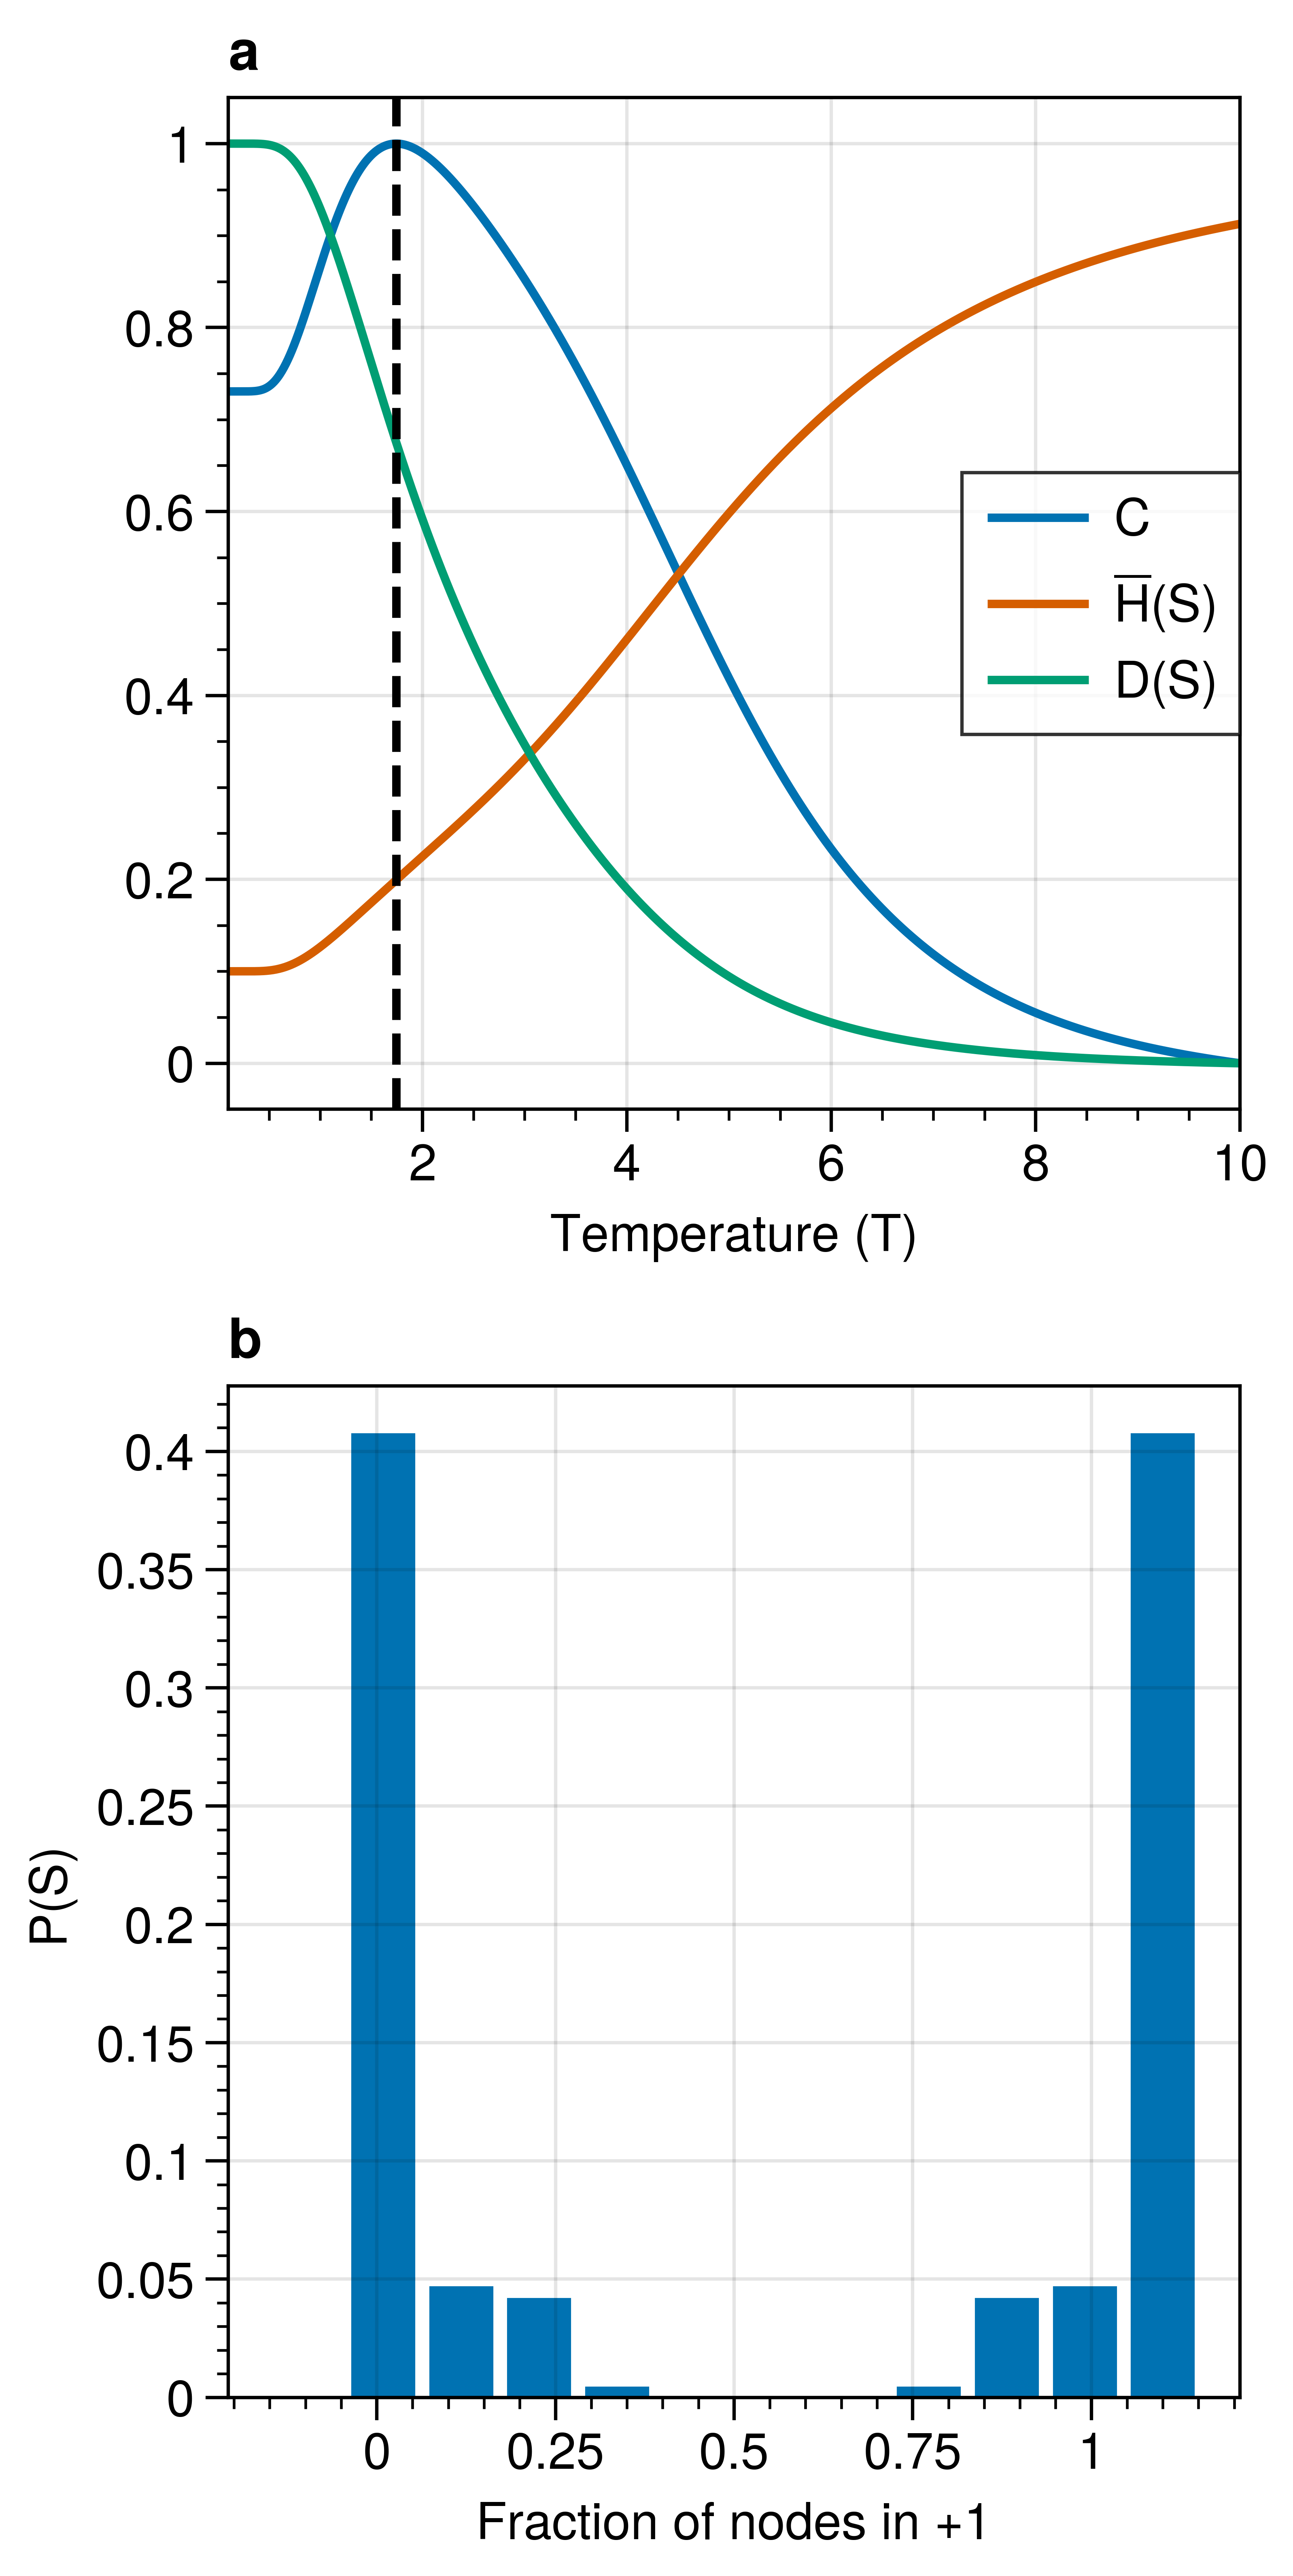
\includegraphics[width=.9\linewidth]{./figures/exact_kite_dyn=ising_beta=0.5732374683235916_T=200_statistical_complexity.png}
\caption{\label{fig:stat_compl}(a) Statistical complexity ($C$), normalized system entropy ($H(S)$) and disequilibrium ($D(S)$) as a function of the temperature ($T = \frac{1}{\beta}$) for Krackhardt kite graph. The noise parameter was set such that it maximizes the statistical complexity (vertical black line). The values are normalized between [0,1] for aesthetic purposes. (b) State distribution $P(S)$ for temperature that maximizes the statistical complexity in (a) as a function of nodes in state +1.}
\end{figure}

\subsection{Exact information flows $I(s_i ; S^t)$}
\label{sec:org59af222}
In   order   to   compute   $\infdecay$,   the   conditional
distribution  $p(S^t  |  s_i)$  and  $p(S^t)$  needs  to  be
computed. For  Glauber dynamics, the system  $S$ transitions
into $S'$ by considering to  flips by randomly choosing node $s_i$. The  transition matrix $P(S^t |  s_i) = \m P$  can be
constructed by computing each entry $p_{ij}$ as

\begin{equation}
\label{eq:glauber}
\begin{split}
p_{ij, i \neq j} &= \frac{1}{|S|} \frac{1}{ 1 + \exp (-\Delta E) }\\
p_{ii} &= 1 - \sum_{j, j \neq i} P_{ij},
\end{split}
\end{equation}

where $\Delta E =  \mathcal{H}(S_j) - \mathcal{H}(S_j)$ encodes the
energy difference of  moving from $S_i$ to  $S_j$. The state
to state transition $\m P$ matrix will be of size $2^{|S|} \times
2^{|S|} \times |\mathcal{A}_{s_i}|$, where $|\mathcal{A}_{s_i}|$ is the size of
the alphabet of $s_i$, which becomes computationally intractable due
to its  exponential growth with  the system size  $|S|$. The
exact information  flows can then be  computed by evaluating
$p(S^t |  s_i)$ out of  equilibrium by evaluating  all $S^t$
for  all  possible  node  states  $s_i$  where  $p(S^t)$  is
computed as

\begin{equation}
p(S^t) = \sum_{s_i} p(S^t | s_i ) p(s_i).
\end{equation}

\subsection{White noise estimation procedure}
\label{sec:orgc093508}
Let $M(S^t)$  represent the instantaneous  system macrostate
compute as the system average

\begin{equation}
\label{}
M(S^t) = \frac{1}{|S|} \sum_i s_i.
\end{equation}

The metastable behavior is characterized for the Ising model
by the system fluctuating around two stable points $T1$ with
$M(S) \approx 0$ and $T2$ with $M(S) \approx 1$ for most of the time. By
pinning intervention  the node  is pinned  to the  +0 state,
effectively  biasing the  macrostate $M(S^t)$  towards $T1$.
For any  particular trajectory  the fluctuations  around the
stable points contributed differently for nodes depending on
the nodes embedness  in the system; lower  degree nodes tend
to produce higher fluctuations than higher degree nodes (see
main text). We define the  fluctuations as ``white noise'' and
characterize  the white  noise  as function  of the  pinning
intervention  on   different  nodes.  The  white   noise  is
characterized by  first computing  the set  of windows  $W =
\{w_i  | i\in  1,  \dots  n\}$ where  each  window  $w_i \in  W$
represents  the duration  in  a trajectory  that the  system
state stayed  in either $T1$  or $T2$. Next, the  white noise
was characterized as

\begin{equation}
\label{}
\eta = \frac{1}{|W|} \sqrt{ \sum_j^{|w_i|} (w_{ij} - \overline{w_i})^2},
\end{equation}

where $\overline{w_i}$  is the  average of window  $w_i$ of
the instantaneous  macrostate and  $w_{ij}$ is  a particular
instantaneous state. The white  noise was estimated for $T1$
and $T2$ separately and displayed in \cref{fig:kite_noise}.

\subsection{Switch susceptibility as a function of degree}
\label{sec:org009e10c}
First,  we investigate  the susceptibility  of a  spin as  a
function  of  its  degree.  The  susceptibility  of  a  spin
switching  its  state  is  a function  both  of  the  system
temperature $T$ and the system dynamics. The system dynamics
would   contribute  to   the   susceptibility  through   the
underlying network structure  either directly or indirectly.
The  network  structure  produces local  correlations  which
affects the switch probability for a given spin.

As an initial approximation,  we consider the susceptibility
of a  target spin $s_i$ to  flip from a majority  state to a
minority state  given the state  of its neighbors  where the
neighbors are  not connected among themselves.  Further, the
assumption is that for the instantaneous update of $s_i$ the
configuration of the neighborhood of $s_i$ can be considered
as the  outcome of a  binomial trial.  Let, $N$ be  a random
variable with state space $\{0,  1\}^{|N|}$, and let $n_j \in N$
represent a neighbor of $s_i$.  We assume that all neighbors
of  $s_i$ are  i.i.d.  distributed  given the  instantaneous
system magnetization

\begin{equation}
M(S^t) = \frac{1}{|S^t|} \sum_i s_i^t.
\end{equation}

Let the minority  state be 1 and the majority  state be 0,
the expectation of $s_i$ flipping from the majority state to
the minority state is given as:

\begin{align}
\label{majority_flip}
    \begin{aligned}
        E[ p(s_i = 1 | N ) ]_{p(N)} &= \sum_{N_i \in N} p(N_i) p(s_i = 1 | N_i)\\
            &= \sum_{N_i \in  N} \prod_j^{|N_i|} p(n_j) p(s_i  = 1 |N_i)\\
            &=  \sum_{N_i \in N}  {n\choose k} f^k  (1  -
            f)^{n-k}  p(s_i  = 1 | f), \\
    \end{aligned}
\end{align}

where $f$ is  the fraction of nodes in  the majority states,
$n$ is the  number of neighbors, $k$ is the  number of nodes
in state 0. In figure \cref{fig:maj_flip}. this is computed
as a  function of the  degree of  spin $s_i$. As  the degree
increases,   the  susceptibility   for   a  spin   decreases
relatively  to  the same  spin  with  a lower  degree.  This
implies  that   the  susceptibility  of  change   to  random
fluctuations are  more likely  to occur  in nodes  with less
external constraints as measured by degree.

%CvE Figuur hier geplaatst om de hoofdtekst wat helderder te houden
\section{Information flows with SIS  dynamics}

\begin{figure*}[hbt]
\centering
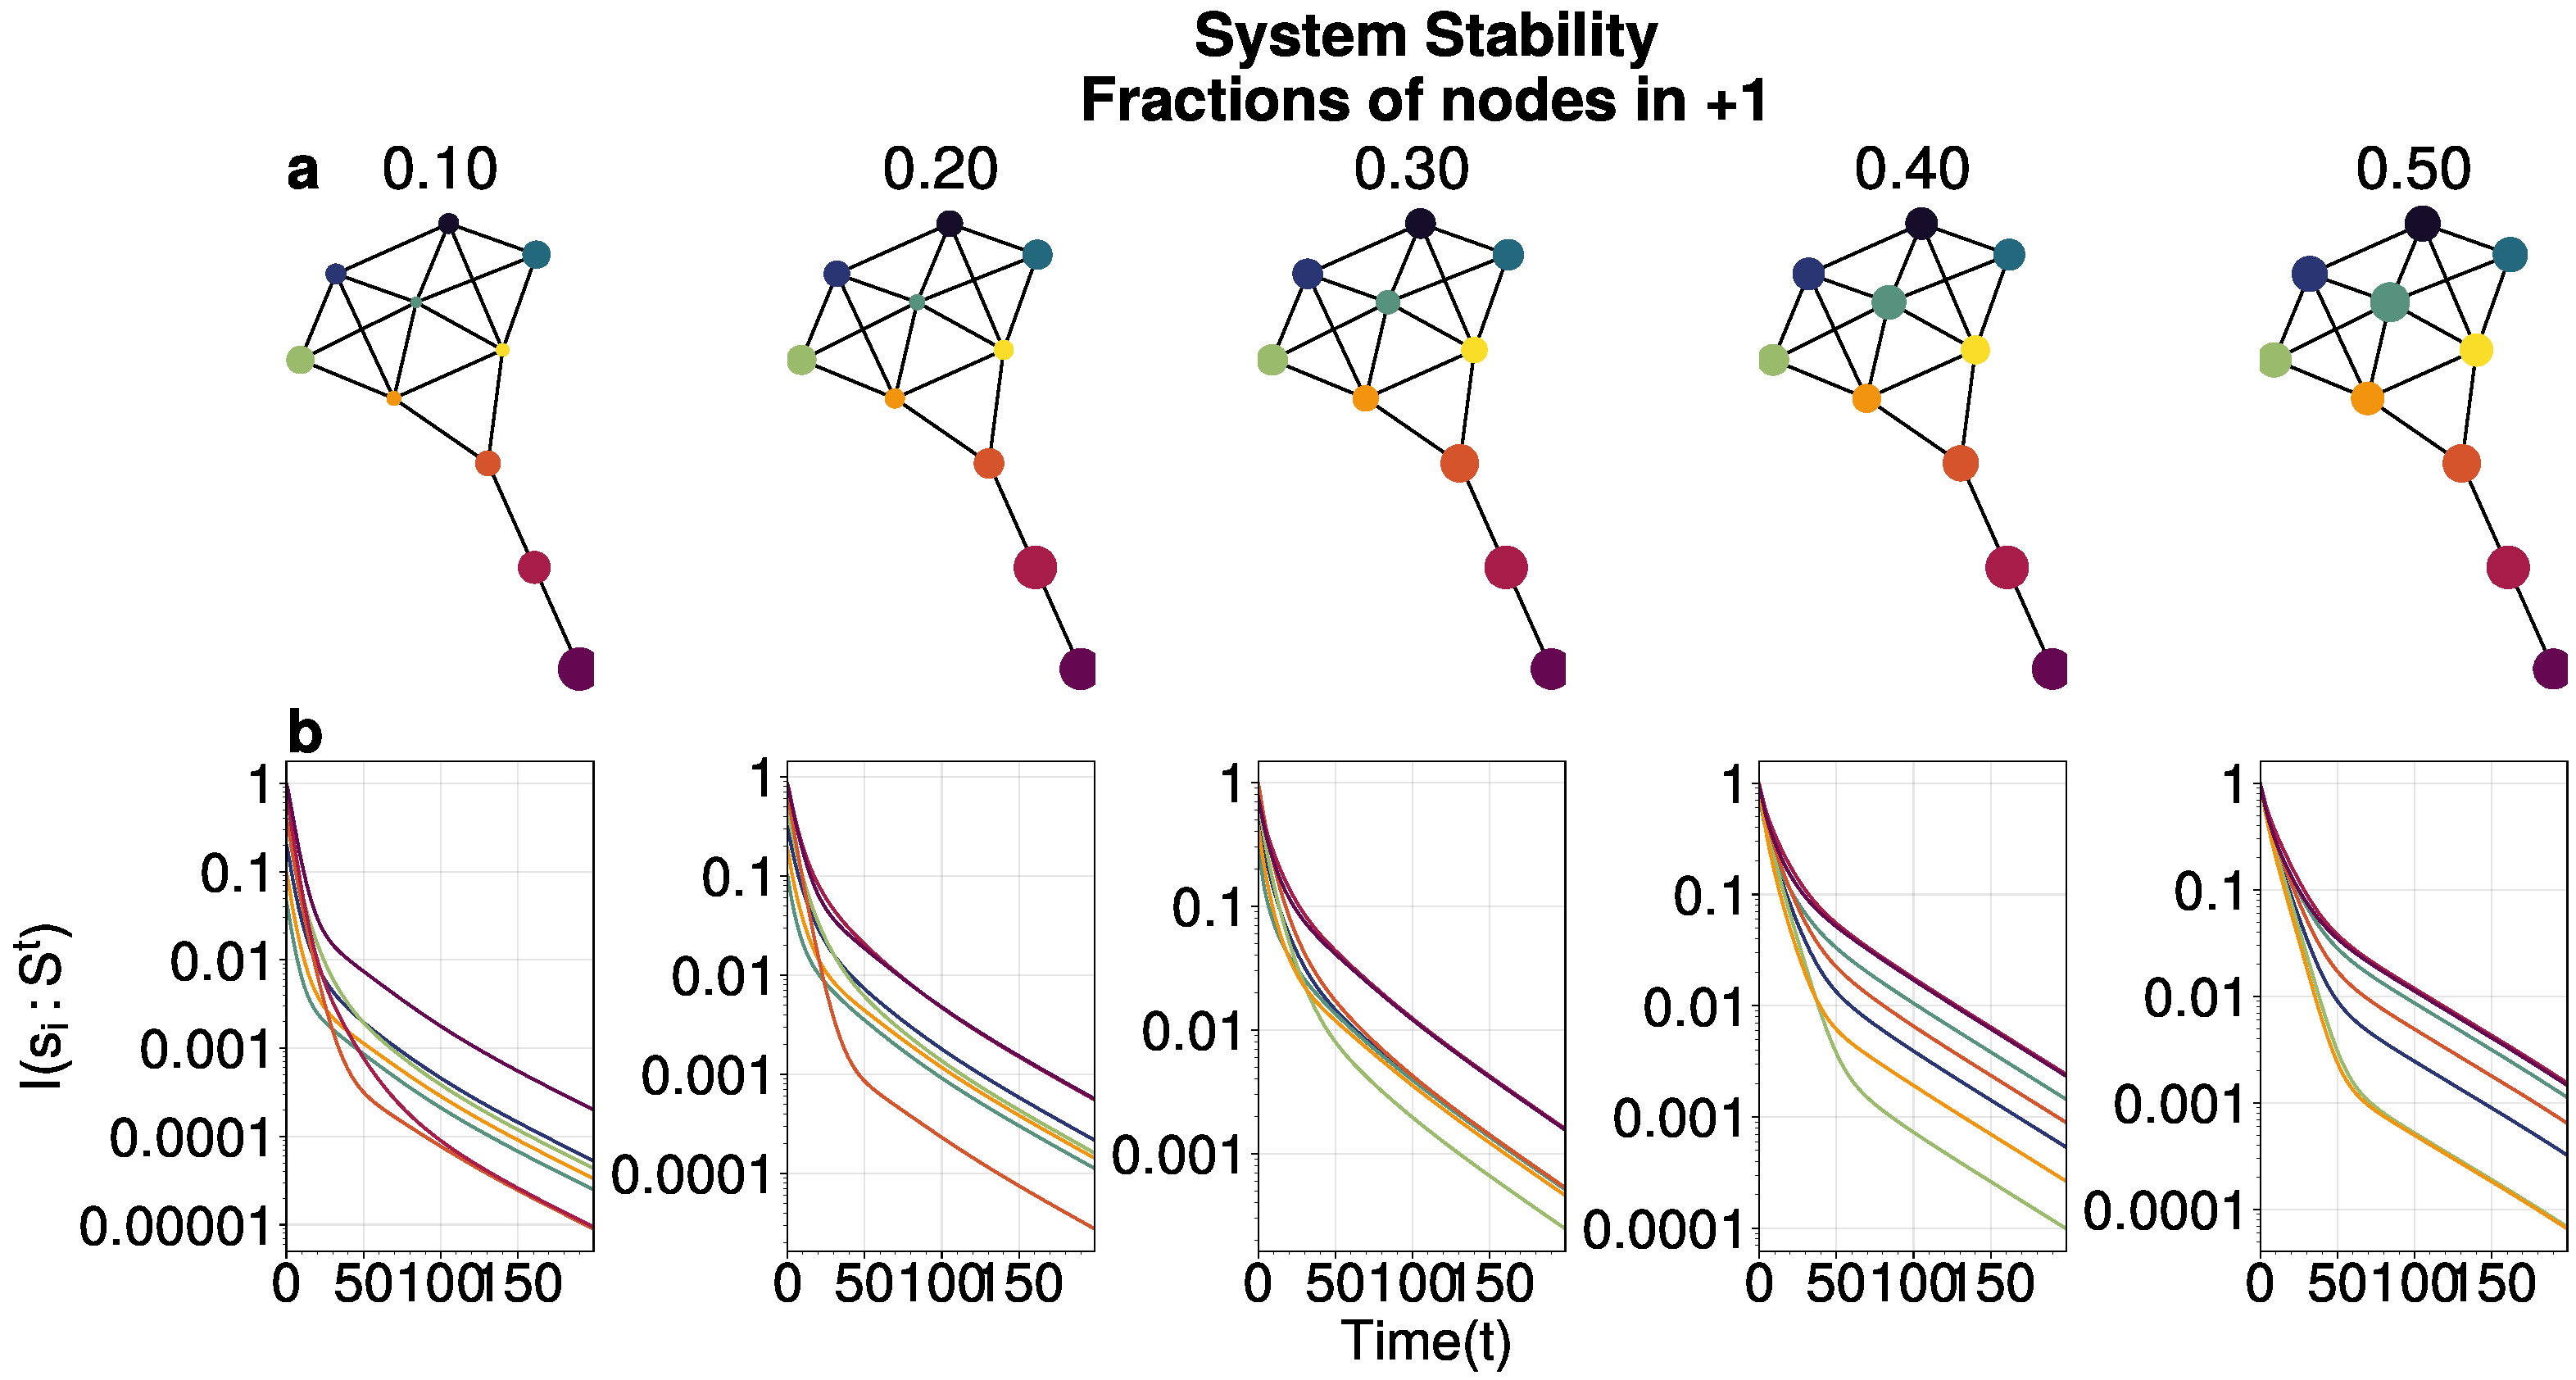
\includegraphics[width=.9\linewidth]{./figures/sis_kite_graph.pdf}
\caption{\label{fig:kite_res_sis}(a) As the system approaches the tipping point the information processing moves from lower degree  nodes to higher degree nodes. Each node is governed by Suseptible-Infective-Susceptible dynamics with infection rate = 0.1, and recovery rate = 0.1. The node size is proportional to the adjusted integrated mutual information. (b) Information flows as a function of system stability. Far from the tipping point the information processing is mainly in lower degree nodes. As the system approaches the tipping point, the information flows increases for all nodes. Higher degree nodes tend to have higher adjusted integrated mutual information and higher information offset. The information offset encodes the long-time scale correlation of the node with the system state. A higher asymptotic information implies that the system remembers the node state for longer than other nodes.}
\end{figure*}

\section{Additional networks}
The kite graph was chosen as it allowed for computing exact information flows while retaining a high variety of degree distribution given the small size. Other networks were also tested. In \cref{fig:other_systems}) different network structure were used. Each node is governed by kinetic Ising spin dynamics.

\begin{figure*}
\centering
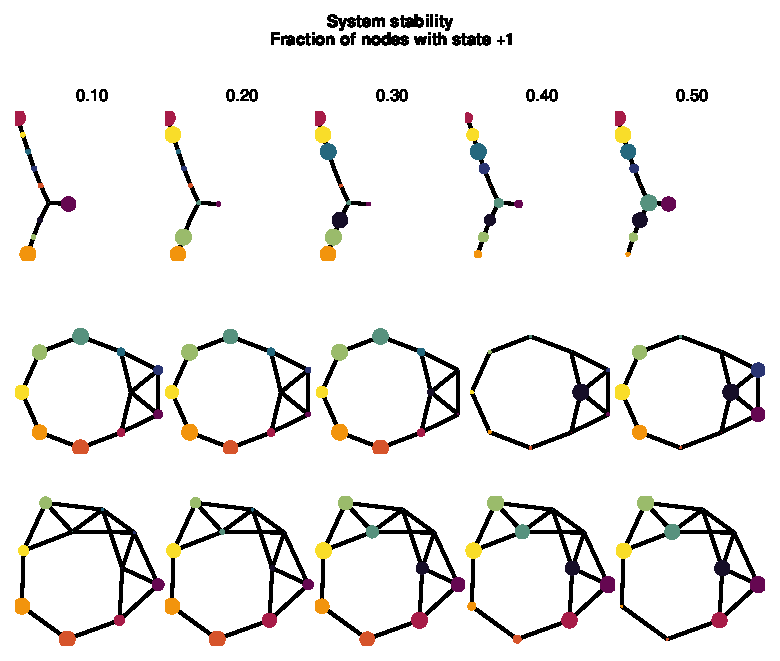
\includegraphics[width=.9\linewidth]{./figures/imi_other_graphs.pdf}
\caption{\label{fig:other_systems}Adjusted mutual information for a random tree (top), and Leder-Coxeter Fruchte graphs (middle, bottom). Each node is goverened by kinetic Ising spin dyanmics. Far away from the tipping point (fraction nodes +1 = 0.5) most information flows are concentrated on non-hub nodes. As the system approaches the tipping point (fraction = 0.5), the information flows move inwards, generating higher adjusted integrated mutual information for nodes with higher degree.}
\end{figure*}





\section{Flip probability per degree}
\label{sec:deg_flip}
%CvE: "semi-meanfield" is nu niet meer deel van de main text
In \cref{fig:maj_flip}  the tendency for a  node to flip
from  the majority  to  the minority  state  is computed  as
function of fraction of nodes possessing the majority states
+1 in the  system, denoted as $N$. Two  things are observed.
First, nodes with lower degree are more susceptible to noise
than nodes with higher degree.  For a given system stability,
nodes with lower degree tend  to have a higher tendency
to flip. This is true for all distances of the system to the
tipping point.  In contrast,  the higher  the degree  of the
node, the closer the system has to be to a tipping point for
the node to  change its state. This can be  explained by the
fact that lower degree nodes, have fewer constraints compared
to nodes with higher degree  nodes. For Ising spin kinetics,
the nodes  with higher  degree tend to  be more  ``frozen'' in
their node dynamics than nodes with lower degree. Second, in
order for a node to flip with probability with similar mass,
i.e. ($E[p(s_i) |  N] = 0.2$) a node with  higher degree needs
to  be closer  to the  tipping point  than nodes  with lower
degree. In  fact, the order of  susceptibility is correlated
with   the  degree;   the   susceptibility  decreases   with
increasing degree and fixed fraction of nodes in state 1.

\begin{figure}[htbp]
\centering
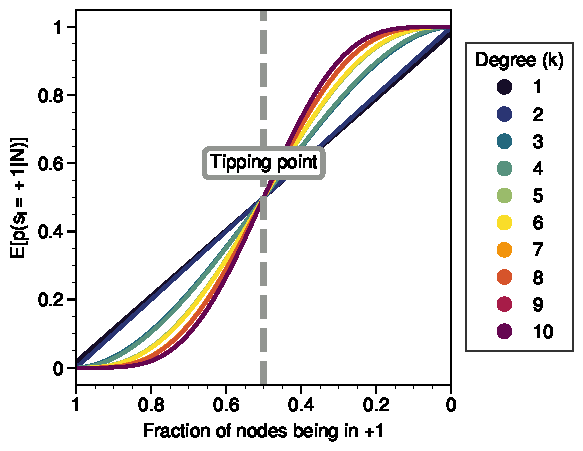
\includegraphics[width=.9\linewidth]{./figures/fig_majority_flip.pdf}
\caption{\label{fig:maj_flip}Susceptibility of a node with degree $k$ switching from the minority state 0 to the majority state 1 as a function of the neighborhood entropy for $\beta = 0.5$. The neighborhood entropy encodes how stable the environment of a spin is. As the system approaches the tipping point, the propensity of a node to flip from to the minority state increases faster for low degree nodes than for high degree nodes. Higher degree nodes require more change in their local environment to flip to the majority state. See for details \ref{sec:org009e10c}.}
\end{figure}


\begin{figure*}[htbp]
\centering
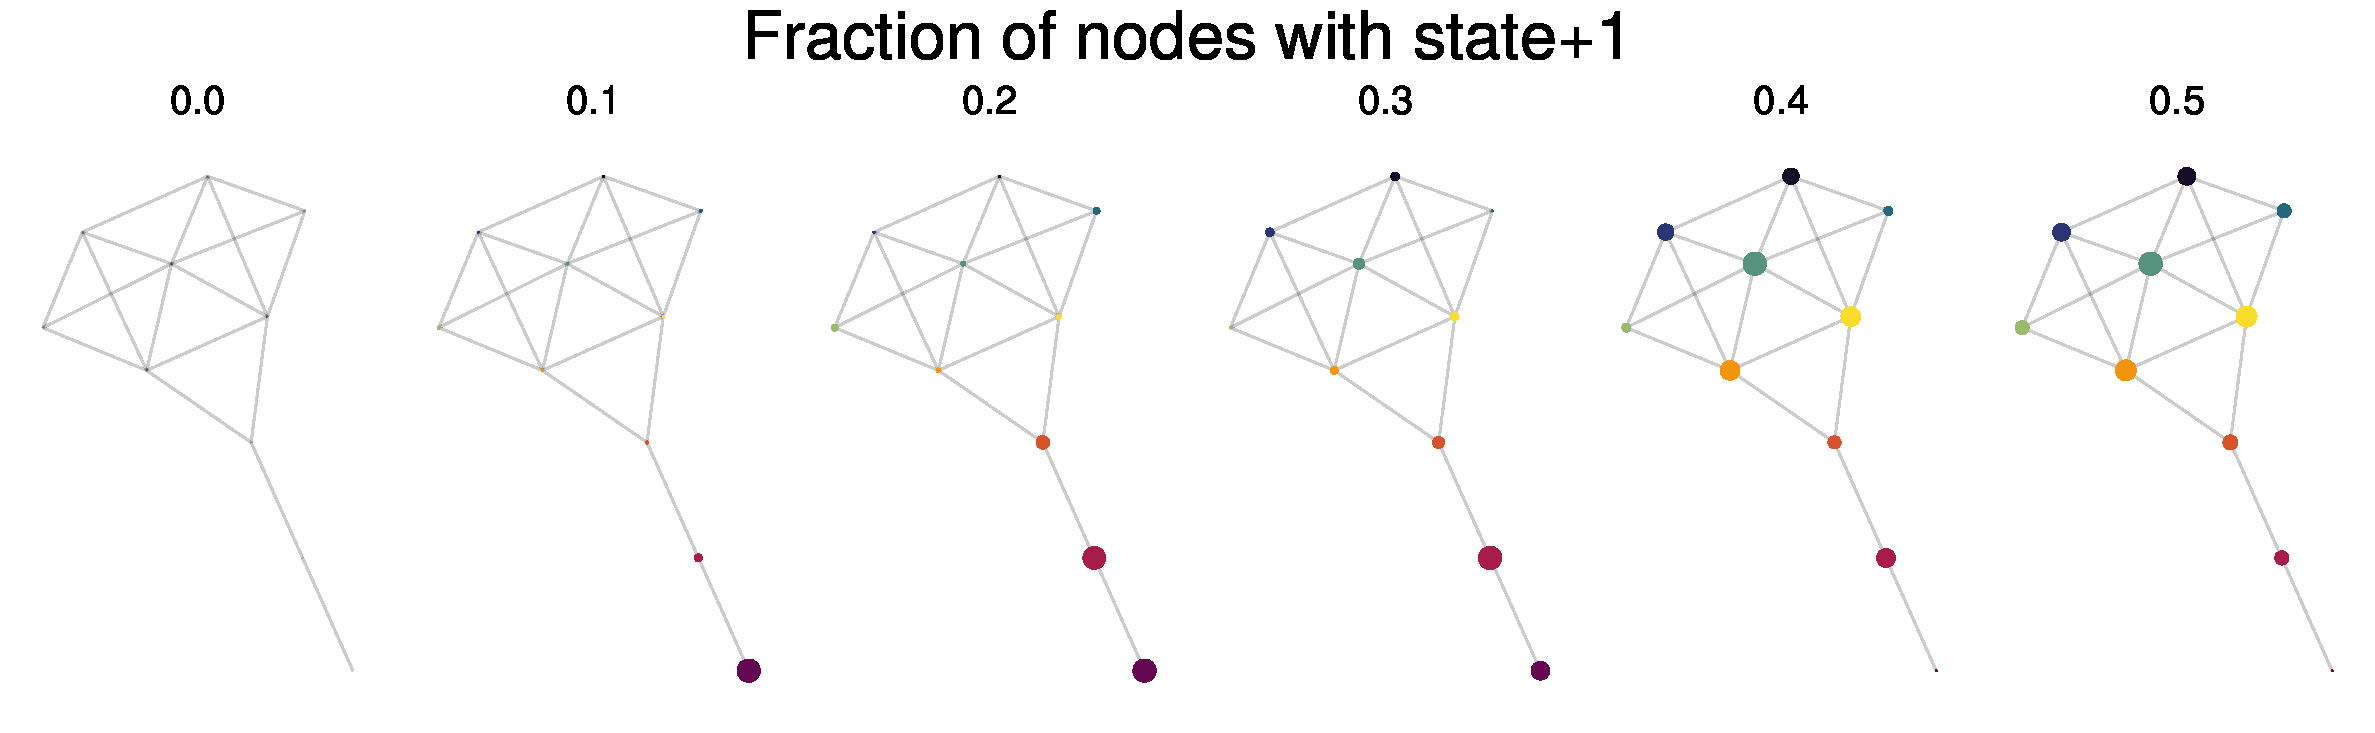
\includegraphics[width=.9\linewidth]{./figures/expectation_kite.pdf}
\caption{\label{fig:expectation_kite} Shortest path analysis of the system ending up in the tipping point from the state where all nodes have state +0. The node size is proportional to the expectation value of a node having state +1  ($E[s_i = 1]_{S^t, M(S^5)}$ as a function of the fraction of nodes having state +1. The expectation values are computed based on 30240 trajectories, an example trajectory can be seen in \cref{fig:max_trajectory}
}
\end{figure*}


\end{document}
